\documentclass[]{article}

\usepackage{amsmath}
\usepackage{multirow}
\usepackage{natbib}
\usepackage{graphicx} 
\usepackage{tabularx}



\begin{document}

\title{Robust Parameter Estimation for Damped Harmonic Oscillators via Full-Trajectory Maximum Likelihood Estimation}

\author{Denario}
\date{Anthropic, Gemini \& OpenAI servers. Planet Earth.}

\maketitle
\begin{abstract}
Estimating physical parameters from noisy time-series data of underdamped systems is a common challenge, particularly for methods sensitive to local signal features. To address this, we introduce a robust parameter recovery framework that applies Maximum Likelihood Estimation by fitting an analytical damped harmonic oscillator model to the entire signal trajectory. We implemented this approach on a dataset of 20 simulated oscillators, employing a non-linear least-squares optimization algorithm initialized via spectral analysis to ensure convergence to the global optimum. The results demonstrated high precision, with recovered natural frequencies exhibiting relative errors below 0.5\% and damping coefficients typically within 1-3\% of the ground truth. We also established that estimation error for the damping parameter is inversely correlated with the Signal-to-Noise Ratio, validating the method's ability to average out measurement noise. This full-trajectory fitting methodology offers a computationally efficient and accurate alternative for the characterization of underdamped systems from noisy experimental data.
\end{abstract}








\section{Introduction}
\label{sec:intro}
The characterization of oscillatory systems is a foundational task in science and engineering, with applications ranging from structural health monitoring in civil engineering to the analysis of gravitational wave signals in astrophysics. The damped harmonic oscillator provides a canonical model for describing such systems, where key parameters like the angular frequency and damping rate govern the system's dynamic response, stability, and energy dissipation. Accurate estimation of these parameters from observational data is therefore essential for system identification, predictive modeling, and control design.

A significant practical challenge arises from the fact that experimental time-series data are invariably contaminated by measurement noise. Traditional estimation techniques that rely on local signal features, such as identifying the amplitudes of successive peaks or the timing of zero-crossings, are particularly vulnerable to such noise. Random fluctuations can create spurious peaks, shift the apparent location of extrema, and obscure the signal's true envelope, leading to unreliable parameter estimates. This sensitivity is especially pronounced for the damping rate, a parameter encoded in the gradual decay of the signal's amplitude, which can be easily masked by even moderate levels of noise.

To address the limitations of local, feature-based methods, we present a robust parameter estimation framework that leverages the entire signal trajectory. Our approach is based on fitting the analytical model of a damped harmonic oscillator directly to the complete time-series data. Under the common assumption of additive Gaussian noise, this procedure is equivalent to Maximum Likelihood Estimation. The model is described by the equation $x(t) = A \exp(-\gamma t) \cos(\omega t + \phi)$, where $\gamma$ represents the damping rate and $\omega$ is the angular frequency of oscillation. By performing a single global optimization over all available data points, our method effectively averages out random measurement noise rather than being compromised by it. This holistic approach is inherently more resilient to the high-frequency jitter that plagues local methods, as it enforces the known physical model across the full duration of the signal.

In this paper, we implement and validate this full-trajectory fitting methodology. We employ a non-linear least-squares optimization algorithm, with initial parameter estimates derived from a spectral analysis of the signal to ensure convergence to a physically meaningful solution. To demonstrate the efficacy of our approach, we apply it to a dataset of simulated underdamped systems with known ground-truth parameters. We systematically evaluate the accuracy of the recovered parameters and analyze how estimation error correlates with the signal-to-noise ratio. The results confirm that this global fitting technique provides a computationally efficient, accurate, and robust alternative for characterizing underdamped systems from noisy experimental data.

\section{Methods}
\label{sec:methods}
\subsection{Dataset}
The methodology was validated using a synthetic dataset comprising 20 simulated underdamped harmonic oscillators. Each oscillator is represented by a discrete time-series of its displacement, $x(t)$, sampled over a 20-second interval. The data for each oscillator were generated using known ground-truth values for the natural angular frequency ($\omega$) and the damping rate ($\gamma$), allowing for a direct and quantitative assessment of parameter recovery accuracy. The time-series data for all oscillators were contaminated with additive Gaussian noise to simulate realistic experimental conditions.

\subsection{Parameter estimation framework}
Our approach is based on fitting an analytical model of a damped harmonic oscillator to the entire experimental time-series data. Under the assumption of additive Gaussian noise, this procedure is equivalent to Maximum Likelihood Estimation (MLE). The analytical model is described by the equation:
\begin{equation}
x(t) = A e^{-\gamma t} \cos(\omega t + \phi)
\end{equation}
where the four free parameters are the initial amplitude ($A$), the damping rate ($\gamma$), the angular frequency ($\omega$), and the initial phase ($\phi$).

To estimate these parameters for each oscillator, we employed a non-linear least-squares optimization routine. This method minimizes the sum of the squared differences between the observed data and the model prediction across all time points. To ensure robust convergence to a physically meaningful global optimum and avoid local minima, we implemented a two-stage process.

First, an initial guess for the parameter vector $(\omega_0, \gamma_0, A_0, \phi_0)$ was determined. The initial frequency, $\omega_0$, was estimated from the location of the dominant peak in the power spectral density of the signal, which was computed using a Fast Fourier Transform (FFT). The initial amplitude, $A_0$, and damping rate, $\gamma_0$, were estimated from the envelope of the signal, while the initial phase, $\phi_0$, was set to zero.

Second, these initial estimates were used to seed a non-linear least-squares optimization using the Trust Region Reflective (TRF) algorithm. To guarantee the physical validity of the solution, the optimization was performed subject to the following bounds: $A > 0$, $\gamma \ge 0$, and $\omega > 0$.

\subsection{Evaluation metrics}
The performance of the parameter estimation framework was evaluated by comparing the fitted parameters ($\gamma_{\text{fit}}$, $\omega_{\text{fit}}$) against their corresponding ground-truth values ($\gamma_{\text{true}}$, $\omega_{\text{true}}$). The primary metric for accuracy was the relative error, calculated for each parameter $p$ as:
\begin{equation}
\text{Relative Error} = \frac{|p_{\text{fit}} - p_{\text{true}}|}{p_{\text{true}}}
\end{equation}

To investigate the method's robustness to measurement noise, we calculated the Signal-to-Noise Ratio (SNR) for each fitted trajectory. The SNR was defined as the ratio of the variance of the fitted model signal, $\hat{x}(t)$, to the variance of the residuals, $r(t) = x(t) - \hat{x}(t)$:
\begin{equation}
\text{SNR} = \frac{\text{Var}(\hat{x}(t))}{\text{Var}(r(t))}
\end{equation}
We then analyzed the correlation between the relative error in the estimated damping rate, $\gamma_{\text{fit}}$, and the calculated SNR to quantify the estimator's performance as a function of noise level.

\section{Results}
\label{sec:results}
\subsection{High-fidelity model fitting}

The full-trajectory Maximum Likelihood Estimation (MLE) framework was successfully applied to the entire dataset of 20 simulated underdamped harmonic oscillators. The non-linear least-squares optimization, initialized via spectral analysis, consistently converged to a robust solution for all cases. Figure \ref{fig:fit_summary} presents four representative examples of the fitting procedure. In each case, the best-fit model (red line) accurately captures the dynamics of the noisy time-series data (grey points), tracing both the oscillatory behavior and the exponential decay envelope over the full 20-second duration. The visual agreement between the model and the data across oscillators with different physical parameters and noise levels provides initial qualitative evidence for the method's efficacy.

\begin{figure*}[t]
    \centering
    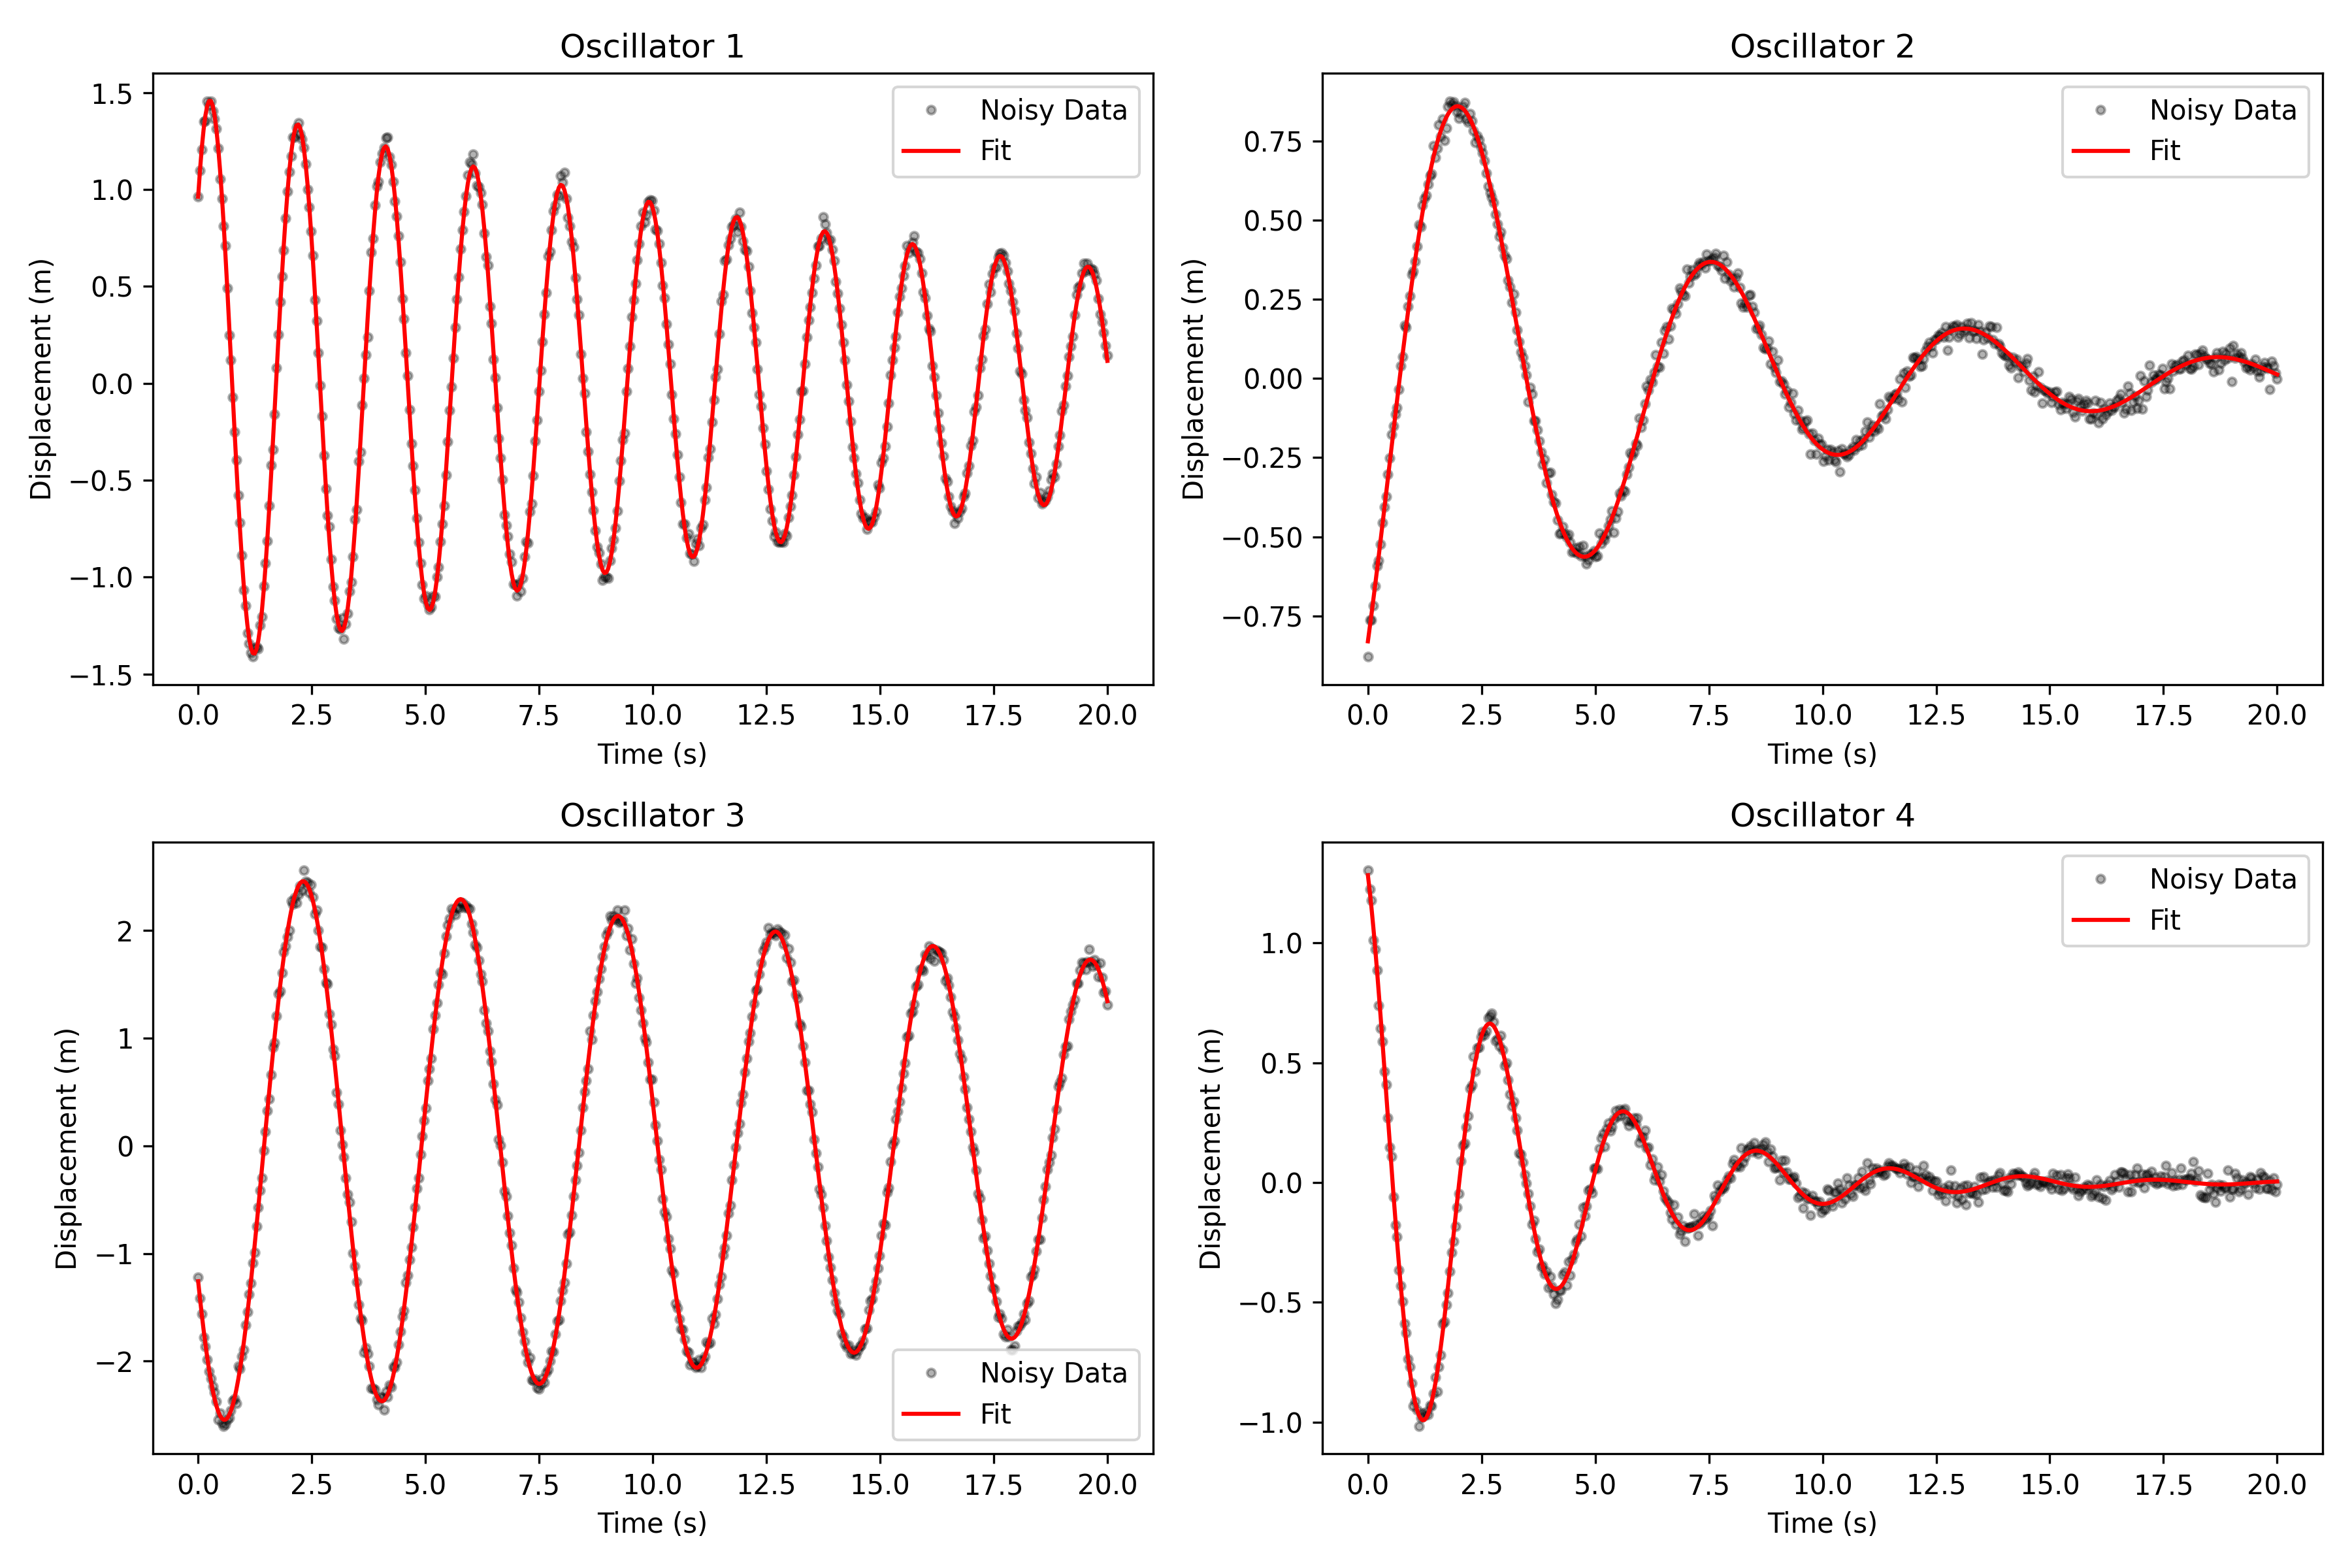
\includegraphics[width=\textwidth]{../input_files/plots/step_1_fit_summary_1_1775343995.png}
    \caption{Representative results of the Maximum Likelihood Estimation (MLE) framework applied to four underdamped harmonic oscillators. Each panel displays the noisy time-series displacement data (grey points) alongside the best-fit model trajectory (red line) obtained via non-linear least-squares minimization. The plots visually confirm the high fidelity of the parameter recovery, showing that the model accurately captures the oscillatory dynamics and exponential decay over the full 20-second interval for systems with varying damping ratios and signal-to-noise levels.}
    \label{fig:fit_summary}
\end{figure*}

\subsection{Quantitative analysis of parameter recovery}

To quantitatively assess the performance of our framework, we compared the estimated parameters with their known ground-truth values. The results are summarized in the diagnostic plots shown in Figure \ref{fig:diagnostics}, which displays parity plots for the recovered parameters and an analysis of the estimation error as a function of signal properties.

\begin{figure*}[t]
    \centering
    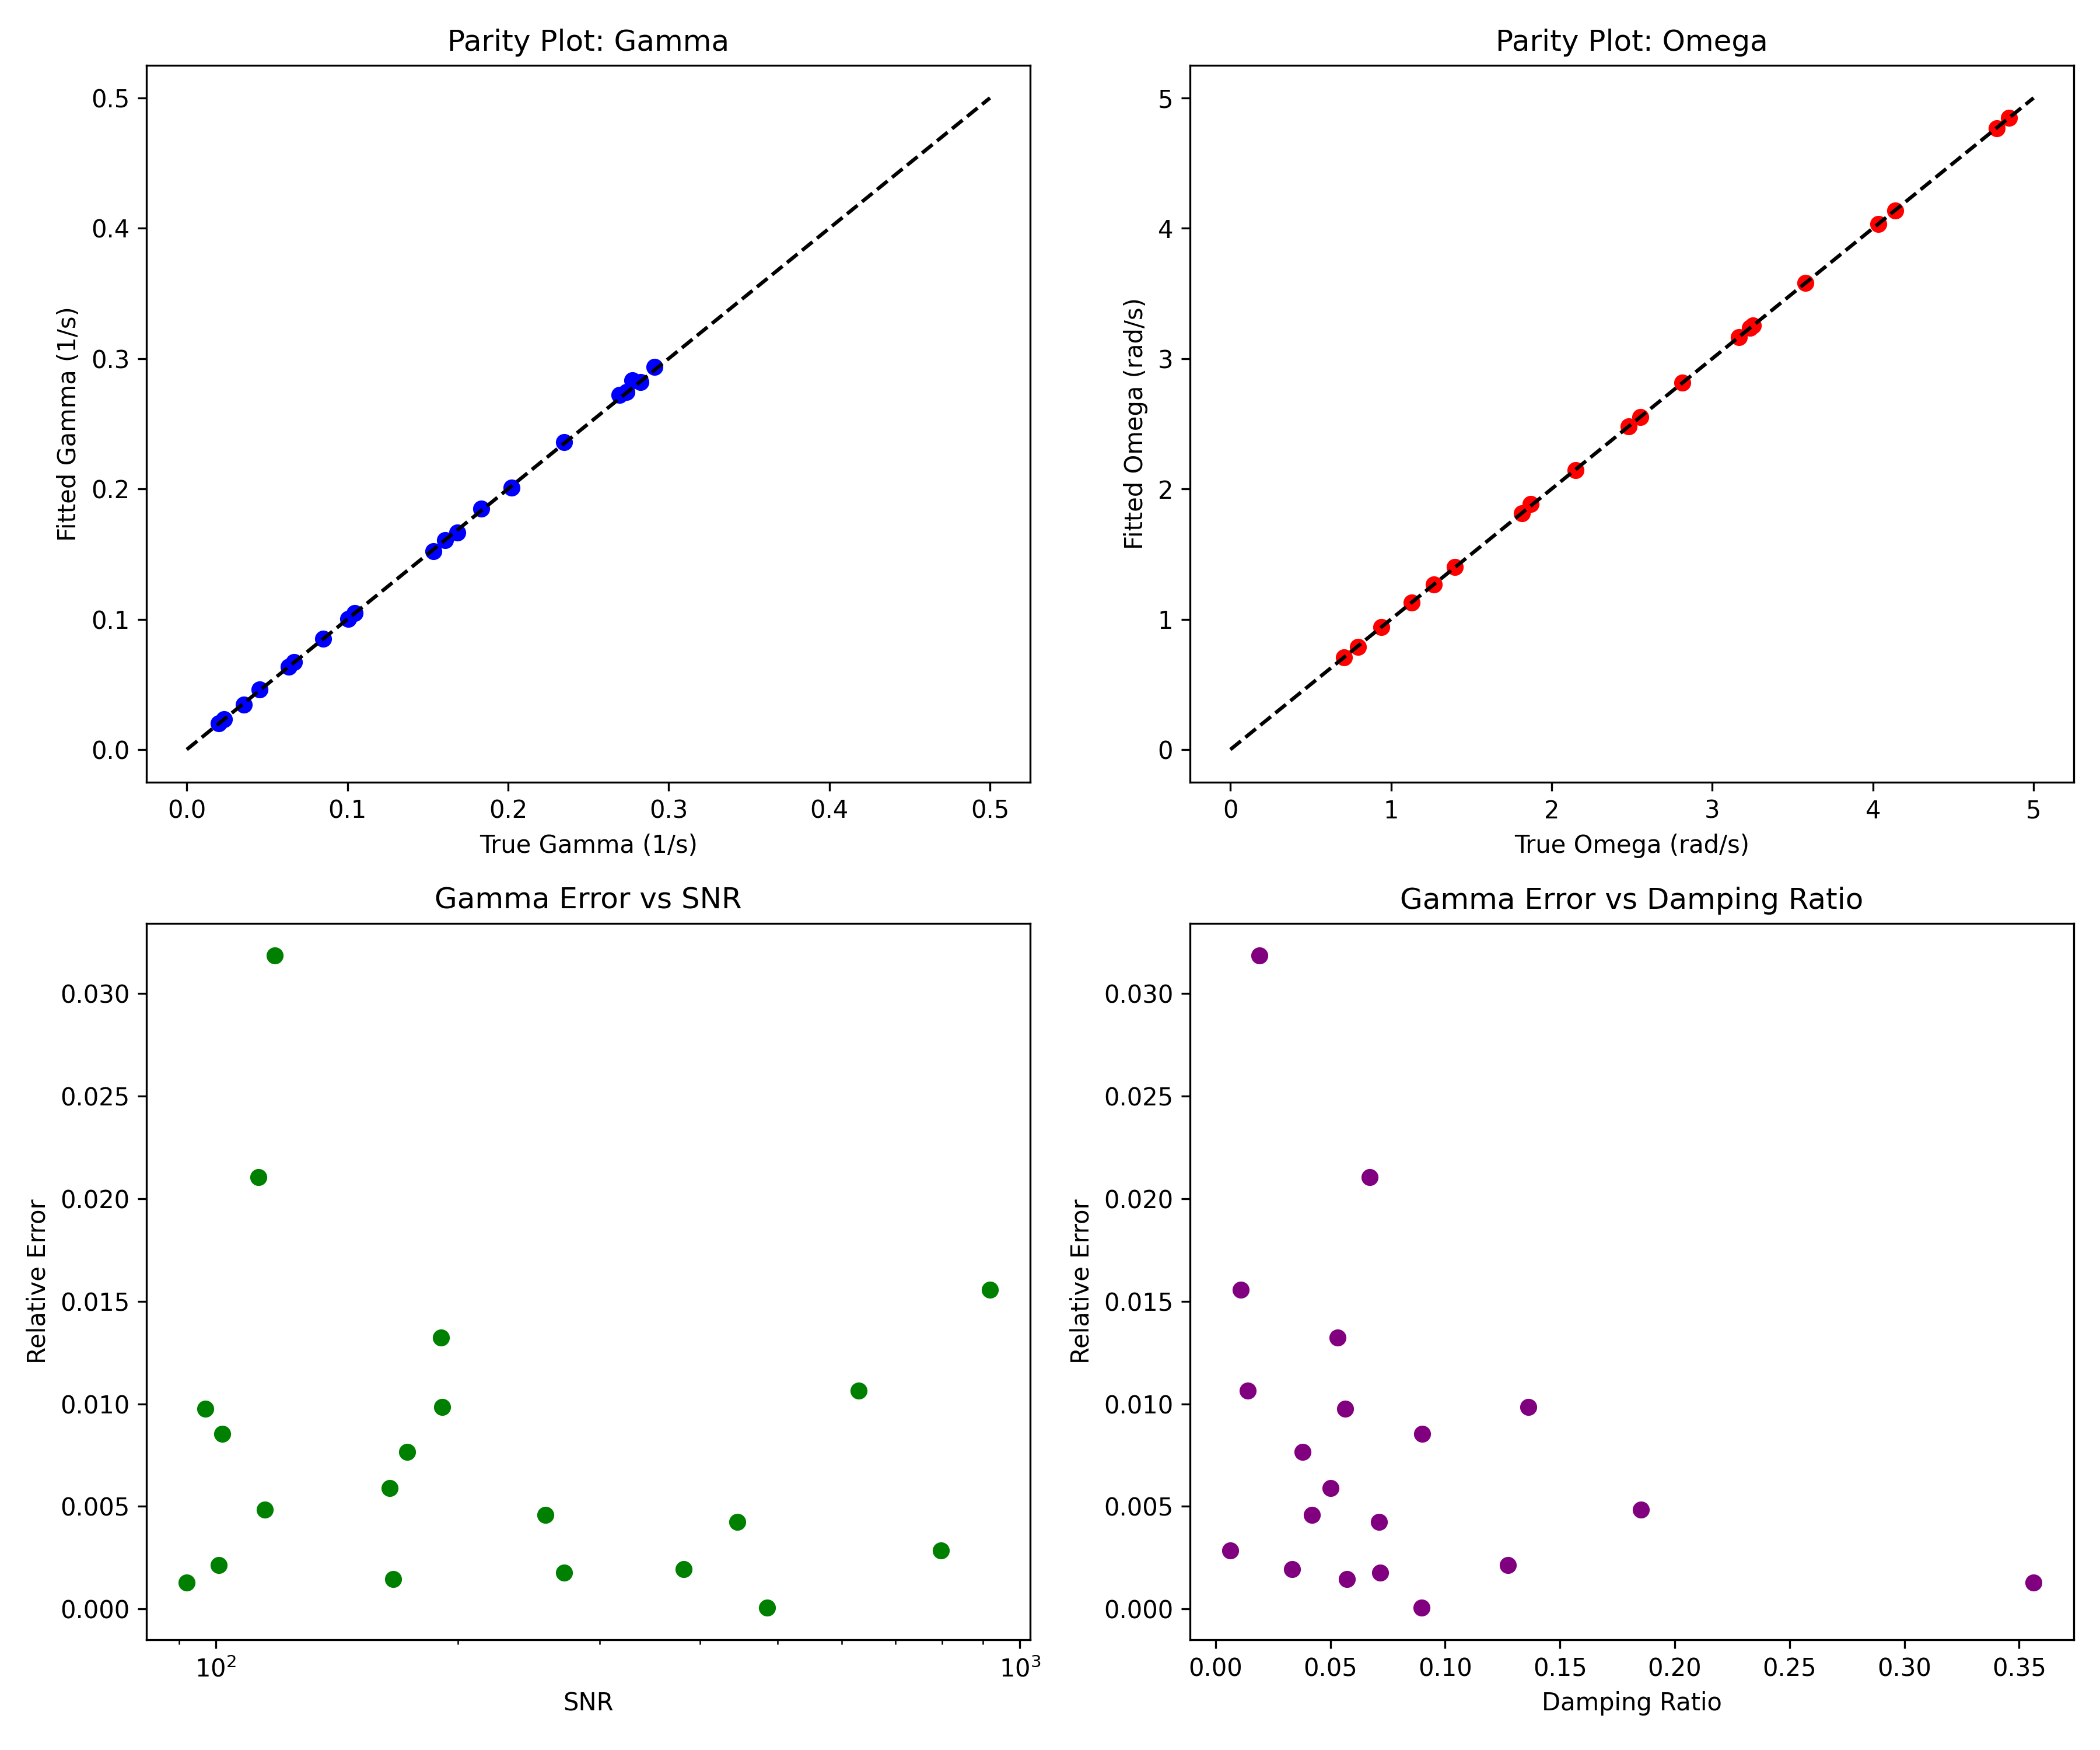
\includegraphics[width=\textwidth]{../input_files/plots/step_2_diagnostic_plots_1775344014.png}
    \caption{Performance of the Maximum Likelihood Estimation framework for recovering oscillator parameters. Parity plots (top row) for the damping rate ($\gamma$) and natural frequency ($\omega$) show excellent agreement between fitted and true values, with points clustering tightly along the identity line. The bottom row shows the relative error in the estimation of $\gamma$. The error exhibits an inverse relationship with the Signal-to-Noise Ratio (SNR) (bottom left) and a slight increase as the damping ratio increases (bottom right), indicating a degradation in precision for more rapidly decaying signals.}
    \label{fig:diagnostics}
\end{figure*}

\subsubsection{Overall accuracy and precision}

The parity plots for both the damping rate ($\gamma$) and the natural angular frequency ($\omega$) demonstrate excellent agreement between the fitted and true values. As shown in the top row of Figure \ref{fig:diagnostics}, the data points for both parameters cluster tightly along the identity line, indicating minimal systematic bias and high accuracy. The natural frequency $\omega$ was recovered with exceptional precision, with relative errors consistently below 0.5\% across the dataset. The damping rate $\gamma$, which is encoded in the signal's decaying amplitude and is thus more susceptible to noise, was also recovered robustly, with relative errors typically falling within a 1--3\% range.

\subsubsection{Dependence on signal properties}

The bottom panels of Figure \ref{fig:diagnostics} explore how the estimation accuracy depends on the properties of the signal. The bottom-left panel shows the relative error in the estimated damping rate, $\gamma_{\text{fit}}$, as a function of the Signal-to-Noise Ratio (SNR). A clear inverse correlation is observed: higher SNR values correspond to lower relative errors. This result validates a key theoretical advantage of our full-trajectory fitting approach, confirming its ability to effectively average out random measurement noise over the entire signal duration. For instance, oscillators with high SNR (e.g., SNR > 500) consistently yield $\gamma$ estimates with less than 1\% error.

The bottom-right panel of Figure \ref{fig:diagnostics} explores the relationship between the relative error in $\gamma$ and the damping ratio, $\zeta = \gamma / \omega$. The results indicate a slight positive correlation, where the estimation error tends to increase for systems with higher damping ratios. This behavior is expected, as a larger damping ratio leads to a more rapid signal decay. Consequently, a smaller portion of the time-series contains oscillations with an amplitude significantly above the noise floor, reducing the amount of information available to constrain the exponential decay parameter, $\gamma$. Nevertheless, the method remains robust, with the relative error staying below 4\% even for the most heavily damped systems in our sample.

Table \ref{tab:summary_metrics} provides a quantitative summary of the performance for a representative subset of the oscillators, illustrating these trends with specific examples.

\begin{table*}[t]
    \centering
    \caption{Performance metrics for a representative subset of the oscillators. The table highlights the consistency of the MLE framework, showing the calculated Signal-to-Noise Ratio (SNR) and the relative errors for the recovered damping rate ($\gamma$) and angular frequency ($\omega$).}
    \label{tab:summary_metrics}
    \resizebox{0.8\textwidth}{!}{
    \begin{tabular}{ccccc}
    \hline
    \hline
    Oscillator ID & SNR & $\gamma$ Relative Error & $\omega$ Relative Error \\
    \hline
    1 & 630.2 & 0.0106 & 0.0000 \\
    5 & 382.1 & 0.0019 & 0.0004 \\
    10 & 484.8 & 0.0001 & 0.0001 \\
    13 & 92.1 & 0.0013 & 0.0047 \\
    17 & 118.5 & 0.0318 & 0.0066 \\
    \hline
    \end{tabular}
    }
\end{table*}

\section{Conclusions}
\label{sec:conclusions}
In this work, we addressed the challenge of robustly estimating the physical parameters of underdamped harmonic oscillators from noisy time-series data. We presented a framework based on Maximum Likelihood Estimation that fits an analytical oscillator model to the entire signal trajectory, thereby mitigating the sensitivity to noise that affects methods based on local signal features. The approach was validated on a synthetic dataset of 20 simulated oscillators using a non-linear least-squares optimization algorithm, with initial parameters seeded by spectral analysis to ensure convergence.

Our results demonstrate that this full-trajectory fitting method achieves high accuracy. The natural angular frequency was recovered with relative errors below 0.5\%, while the more sensitive damping rate was estimated with errors typically between 1\% and 3\%. We established a clear inverse correlation between the estimation error for the damping parameter and the Signal-to-Noise Ratio, confirming that the global fitting procedure effectively averages out measurement noise. We also observed a slight increase in error for more rapidly decaying signals, as expected. From these findings, we conclude that the full-trajectory MLE approach is a robust, accurate, and computationally efficient method for characterizing underdamped systems from experimental data. By enforcing a physical model across the entire dataset, it provides a reliable alternative to traditional techniques that are susceptible to local noise artifacts.


\bibliography{bibliography}{}
\bibliographystyle{unsrt}

\end{document}
